\documentclass[12pt,fleqn]{article}
\setlength{\parindent}{0pt}
\usepackage{graphicx}
\usepackage{cancel}
\usepackage{listings}
\usepackage[latin5]{inputenc}
\usepackage{color}
\setlength{\parskip}{8pt}
\setlength{\parsep}{0pt}
\setlength{\headsep}{0pt}
\setlength{\topskip}{0pt}
\setlength{\topmargin}{0pt}
\setlength{\topsep}{0pt}
\setlength{\partopsep}{0pt}
\setlength{\mathindent}{0cm}
\usepackage{latexsym}
\usepackage{amsfonts}
\usepackage{showkeys}
\renewcommand*\showkeyslabelformat[1]{(#1)}

\begin{document}
Ders 3

Ornek 

Bir onceki ornegin dogal bir uzantisi n-boyutlu reel kordinat uzayi
olabilir. Bu uzaydaki vektorler n-ogeli icinde n tane reel sayi olan bir
dizidirler, ve vektorler $x = (\xi_1, \xi_2,...,\xi_n)$
formundadirlar. Reel tek sayi $\xi_k$'ye vektorun $k$'inci elemani adi
verilir. Iki vektor, eger tum ogeleri birbirine esit ise, esittir. Sifir
vektoru $\theta = (0,0,...,0)$ seklinde tanimlidir. 

$n$ boyutlu reel kordinat uzayi $R^n$ olarak tanimlanir. Buna tekabul eden
n-ogeli kompleks sayilarin uzayi $C^n$'dir. 

Bu noktada aslinda boyut kavramini devreye sokmak icin biraz erken. Daha
ileriki derslerde boyut kavraminin detayli tanimi yapilacak, ve bu
bahsettigimiz uzaylarin hakikaten n-boyutlu oldugu ispatlanacak. 

Ornek 

Sonsuz sayida eleman, sonsuz ogeli dizi iceren vektorlerlerle ilginc bazi
uzaylar insa edilebiliyor, ki bu uzayda tipik bir vektor vektorler 
$x =
(\xi_1, \xi_2,...,\xi_k,...)$ seklinde oluyor. Diger bir sekliyle $x =
\{\xi_k\} _{k=1}^{\infty}$. 
Toplama ve cikartma onceden oldugu gibi teker teker, sirasi birbirine uyan
ogeler arasinda yapiliyor. Reel sayilardan olusan her turlu sonsuz
dizilerin listesi bir vektor uzayi olusturuyor. Bir dizi $\{\xi_k\}$'ye
sinirli (bounded) denir, eger her $k$ icin.  $|\xi_k| < M$ olacak sekilde
bir $M$ sabiti var ise. Sonsuz ve sinirli (tanimini biraz once yaptik) olan 
her dizi bir vektor uzayi olusturur, cunku iki sinirli dizinin birlesimi, ya
da dizinin sayisal carpimi yine bir sinirli dizi olacaktir. 

Ornek 

Icinde sonlu / belirli (finite) miktarda sifira esit olmayan oge iceren tum
dizilerin birlesimi bir vektor uzayidir (her vektor -dizi- icinde farkli
miktarda sifir olmayan oge olabilir). Bu uzaya sonlu sayida sifiri olmayan
dizilerin uzayi ismi verilir. 

Ornek

Sonsuz tane reel sayidan olusan ve hepsi de sifira yaklasan dizilerin
birlesimi bir vektor uzayidir, cunku bu tur sifira yaklasan iki dizinin
toplami da ayni sekilde sifira yaklasir. Boyle bir dizinin skalar ile
'carpimi, yani kati yine sifira yaklasir. 

Ornek 

Reel cizgi uzerinde bir $[a,b]$ araligi dusunun. Bu aralik uzerinde tanimli
tum surekli fonksiyonlar bir vektor uzayi olusturur. Iki vektor $x,y$ daha
detayli olarak $x(t),y(t)$ olarak kullaniliyor, ki $t \in [a,b]$. Eger $x =
y$ ise 
$x(t) = y(t)$ demektir. $(x+y)(t) = x(t) + y(t)$ ve $(\alpha x)(t) =
\alpha x(t)$ kullanilir. 
Sifir vektoru $\theta$ bu aralikta surekli sifir degerinde olan vektordur. 
Bu uzaya [a,b] arasinda reel degerli surekli fonksiyonlar uzayi denir. 

Simdi birkac vektor uzayini birlestirerek nasil daha buyuk bir tane
yaratabilecegimizi gorelim. 

Tanim

$X,Y$'nin ayni skalar alani uzerinden tanimli iki vektor uzayi oldugunu
dusunelim. $X,Y$'nin kartezyen carpimi, ki bu $X \times Y$ olarak
gosterilir, iki ogeli siralanmis bir dizi olusturacaktir, 
yani $(x,y)$, ki $ x \in X, y \in Y$. $X \times Y$ uzerinde toplama ve
skalar carpim $(x_1,y_1) + (x_2,y_2) = (x_1+x_2, y_1+y_2)$ ve
$\alpha(x_1,y_1) = (\alpha x_1,\alpha y_1)$. 

Ustteki tanimin bir vektor uzayi olmanin gerekliliklerini yerine getirdigi
ortadadir. Hatta bu tanim kolaylikla $n$ tane vektor uzayinin kartezyen
carpimina genisletilebilir, yani $X_1,X_2,..,X_n$. Bu carpimi temsil etmek
icin $X^n$ yazacagiz. 

Alt Uzaylar (Subspaces), Lineer Kombinasyonlar, ve Lineer Cesitler (Linear Varieties) 

Tanim 

$M$, $X$'in bos olmayan bir {\em alt uzayidir} (subspace) eger $\alpha x + \beta y$
formundaki her vektor $M$ icinde ise, ve $x,y \in M$ olmak uzere. 

Hicbir alt uzayin bos olmadigini bastan kabul ettigimize gore, icinde en az
bir $x$ olmalidir. Tanim itibariyle ayrica  $0 x = \theta$'yi da
icermelidir, o zaman her alt uzay sifir vektorunu de icerir. En basit alt
uzay icinde sadece $\theta$ olan alt uzaydir. Uc boyutlu uzayda orijinden
gecen bir duzlem bir alt uzay olusturur, orijinden gecen bir cizgi ayni
sekilde bir alt uzay olusturur. 

$X$'in tamami da $X$'in (yani kendisinin) bir alt uzayidir. Tum uzaya esit
olmayan bir alt uzaya duzgun (proper) alt uzay denir. 

Her alt uzay kendi ogelerinin toplamlarini, ve katlarini icerdigi icin ayni
anda bir uzayi tanimlayan 7 gerekliligi (axiom) otomatik olarak yerine
getirmis olur. Zaten alt uzay derken ``uzak'' kelimesini kullanabilmemizin
sebebi budur. 

Diyelim ki $X$ uzayi $n$ ogeli dizinlerin (tuple) birlesimi. Bu dizinlerin
bir kopyasini dusunelim, tek farkla, 1. ogenin hep sifir olsun. Bu bir alt
uzaydir. $1/2$ noktasinda sifir olan $[0,1]$ uzerinde tanimli surekli
fonksiyonlar, tum surekli fonksiyonlarin bir alt uzayidir. 

Iki alt uzayin evliligi (union, $\cup$ ile gosterilen) bir alt uzay
olmayabilir. Bir duzlem uzerinde mesela, ayni yonde gitmeyen (noncolinear)
iki cizginin evliligi, bu iki ayri cizginin rasgele toplamlarini icermedigi
icin alt uzay olma sartini yerine getirmez. Fakat ``kumelerin toplami''
kavramindan hareketle, iki alt uzay daha buyuk bir alt uzay olarak ozel bir
sekilde birlestirilebilir.

Tanim

Bir vektor uzayinin $S,T$ adli iki alt kumesinin toplami $S+T$ olarak
gosterilir, ve her $s+t$ formundaki tum vektorleri icerir, ki $s \in S,t
\in T$ 
olmak uzere. Dikkat, daha $S,T$'nin alt uzay oldugunu soylemiyoruz, sadece
kume diyoruz (simdilik). 

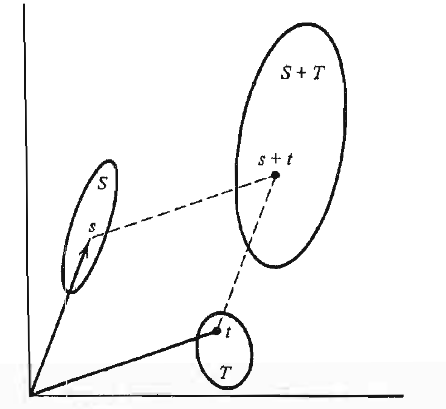
\includegraphics[height=5cm]{3_1.png}

Ustteki resim toplam kavramini iki boyutlu uzayda (ki bu bir vektor
uzayidir) gosteriyor. Vektor uzayi, $S,T$ icindeki noktalara dogru isaret
eden orijinden cikan iki vektoru goruyoruz. Toplam olarak, hakikaten
$S$'teki noktanin / vektorun mesela (3,1) oldugunu dusunsek, $T$'deki
noktanin / vektorun (1,3) oldugunu dusunsek, onlarin toplami olarak
gosterilen nokta kabaca (4,4) gibi duruyor degil mi? Sekil bu kavrami
temsili olarak iyi gostermis. Toplamin ayrica daha buyuk bir kume olduguna
dikkat. 

Teori 

Diyelim ki $M,N$ vektor uzaylari $X$'in birer alt kumesi. O zaman bu kumelerin
toplami $M + N$ ayni sekilde $X$'in bir alt uzayidir. 

Ispat 

$M+N$'nin $\theta$'yi icerdigi bariz. Devam edelim, $x,y \in S+T$ icin
muhakkak 

\[ x = m_1 + n_1 \]

\[ y = m_2 + n_2 \]

var demektir, ki $m_1,m_2 \in M$, $n_1,n_2 \in N$. Bu kume toplami
tanimindan geliyor zaten. 

Simdi $x,y$'yi ayri ayri rasgele sabitler $\alpha,\beta$ ile carpalim. 

\[ \alpha x = \alpha m_1 + \alpha n_1 \]

\[ \beta y = \beta m_2 + \beta n_2 \]

Carpimlari toplayalim

\[ \alpha x + \beta y  = \alpha m_1 + \alpha n_1 + \beta m_2 + \beta n_2 \]

Esitligin sagini tekrar duzenleyelim

\[ \alpha x + \beta y  = (\alpha m_1 + \beta m_2) + (\alpha n_1  + \beta n_2 )\]

$\alpha x + \beta y $ ile $S+T$ icindeki $x+y$'nin herhangi bir sekildeki
katini almis oluyoruz. Ve geldigimiz en son esitlik gosteriyor 
ki $\alpha x
+ \beta y$ yine $M,N$ icindeki vektorlerin katlari kullanilarak 
temsil edilebiliyor. Yani toplamdaki kat islemini aynen alt kumelere
yansitabiliyoruz / onlarin bazinda yapabiliyoruz. O zaman alt kumeler alt
uzay oldugu icin toplam da alt uzay demektir. Ispat tamam.

Iki boyutlu Oklit uzayinda orijinden gecen ve ayni yonde olmayan iki cizginin
toplami tum uzaydir. 

Tanim

Vektor uzayindaki vektorler $x_1,x_2,..,x_n$'in lineer kombinasyonu
$\alpha_1 x_1 + \alpha_2 x_2 + ... + \alpha_n x_n$ olarak gosterilir. 

Daha once vektor toplami iki tane vektorun toplami olarak
gostermistik. Ustteki gibi $n$ tane toplam icin (eski tanima gore) toplam
ikiser ikiser yapilmali tabii. Ve bunun dogal uzantisi olarak, alt
uzaydaki vektorlerin lineer kombinasyonu yine alt uzayda olacaktir. Ters
yonden bakarsak, bir vektor uzayinin herhangi bir alt kumesinin lineer
kombinasyonlarini kullanarak bir alt uzayi yaratabiliriz. 

Tanim

Diyelim ki $S$ vektor uzayi $X$'in bir alt kumesi. {\em S tarafindan
  uretilen alt uzay} yani $[S]$, $S$'teki elemanlarin lineer
kombinasyonu olan $X$'teki vektorlerden olusur. 







\end{document}
